% Created 2022-07-08 Fri 18:14
% Intended LaTeX compiler: pdflatex
\documentclass[presentation,aspectratio=169]{beamer}
\usepackage[utf8]{inputenc}
\usepackage[T1]{fontenc}
\usepackage{graphicx}
\usepackage{grffile}
\usepackage{longtable}
\usepackage{wrapfig}
\usepackage{rotating}
\usepackage[normalem]{ulem}
\usepackage{amsmath}
\usepackage{textcomp}
\usepackage{amssymb}
\usepackage{capt-of}
\usepackage{hyperref}
\usepackage{khpreamble}
\usepackage{amssymb}
\usepackage{tcolorbox}
\DeclareMathOperator{\shift}{q}
\DeclareMathOperator{\diff}{p}
\usetheme{default}
\author{Kjartan Halvorsen}
\date{2022-07-08}
\title{Group exercise on relative stability}
\hypersetup{
 pdfauthor={Kjartan Halvorsen},
 pdftitle={Group exercise on relative stability},
 pdfkeywords={},
 pdfsubject={},
 pdfcreator={Emacs 26.3 (Org mode 9.4.6)}, 
 pdflang={English}}
\begin{document}

\maketitle

\section{Phase margin}
\label{sec:org76bc68e}
\begin{frame}[label={sec:org7db894d}]{The phase margin}
\begin{center}
\includegraphics[width=0.38\linewidth]{../../figures/implane-nyquist-margins}
\end{center}
\begin{itemize}
\item Cross-over frequency: The frequency \(\omega_c\) for which \(|G_o(i\omega)| = 1\).
\item Phase margin: The angle \(\varphi_m\) to the negative real axis for the point where the Nyquist curve intersects the unit circle. \[\varphi_m = \arg G_o(i\omega_c) - (-180\degree) = \arg G_o(i\omega_c) + 180\degree\]
\end{itemize}
\end{frame}


\begin{frame}[label={sec:orgc145c3c}]{Phase margin for the hard disk drive controller}
\footnotesize

  \begin{center}
  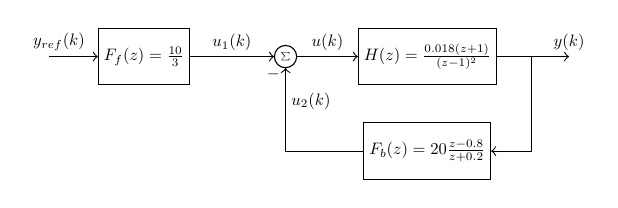
\begin{tikzpicture}[scale=0.6, every node/.style={transform shape}]
  \tikzset{node distance=2cm, 
      block/.style={rectangle, draw, minimum height=12mm, minimum width=14mm},
      sumnode/.style={circle, draw, inner sep=2pt}        
  }

    \node[coordinate] (input) {};
    \node[block, right of=input] (TR) {$F_f(z) = \frac{10}{3}$};
    \node[sumnode, right of=TR, node distance=30mm] (sum) {\tiny $\sum$};
    \node[block,right of=sum, node distance=30mm] (plant) {$H(z) = \frac{0.018(z+1)}{(z-1)^2}$};
    %\node[sumnode, right of=plant, node distance=30mm] (sumdist) {$\sum$};
    %\node[coordinate, above of=sumdist, node distance=15mm] (dist) {};
    %\node[coordinate, right of=sumdist, node distance=15mm] (measure) {};
    \node[coordinate, right of=plant, node distance=30mm] (output) {};
    \node[coordinate, right of=plant, node distance=22mm] (measure) {};
    %\node[sumnode,below of=measure, node distance=25mm] (sumnoise) {$\sum$};
    %\node[coordinate, right of=sumnoise, node distance=15mm] (noise) {};
    \node[block,below of=plant, node distance=20mm] (SR) {$F_b(z)=20\frac{z-0.8}{z+0.2}$};
    \draw[->] (input) -- node[above, pos=0.2] {$y_{ref}(k)$} (TR);
    \draw[->] (TR) -- node[above] {$u_1(k)$} (sum);
    \draw[->] (sum) -- node[above] {$u(k)$} (plant);
    \draw[->] (plant) -- node[at end, above] {$y(k)$} (output);
    \draw[->] (measure) |- (SR);
    \draw[->] (SR) -| (sum) node[right, pos=0.8] {$u_2(k)$} node[left, pos=0.96] {$-$};
  \end{tikzpicture}
  \end{center}

\begin{center}
  \includegraphics[height=0.5\textheight]{../../matlab/harddisk_margin_crop}
  \includegraphics[height=0.5\textheight]{../../matlab/harddisk_nyquist_crop}

\end{center}
\end{frame}


\begin{frame}[label={sec:orgc7d04d4}]{Phase margin with anti-aliasing filter}
\footnotesize

\begin{center}
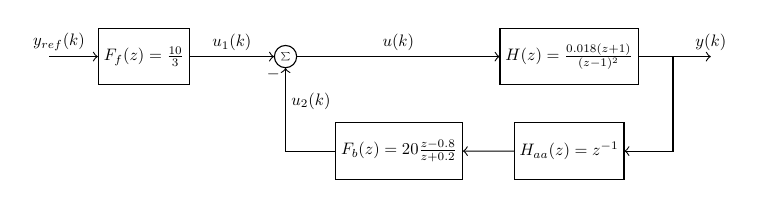
\begin{tikzpicture}[scale=0.6, every node/.style={transform shape}]
\tikzset{node distance=2cm, 
    block/.style={rectangle, draw, minimum height=12mm, minimum width=14mm},
    sumnode/.style={circle, draw, inner sep=2pt}        
}

  \node[coordinate] (input) {};
  \node[block, right of=input] (TR) {$F_f(z) = \frac{10}{3}$};
  \node[sumnode, right of=TR, node distance=30mm] (sum) {\tiny $\sum$};
  \node[block,right of=sum, node distance=60mm] (plant) {$H(z) = \frac{0.018(z+1)}{(z-1)^2}$};
  %\node[sumnode, right of=plant, node distance=30mm] (sumdist) {$\sum$};
  %\node[coordinate, above of=sumdist, node distance=15mm] (dist) {};
  %\node[coordinate, right of=sumdist, node distance=15mm] (measure) {};
  \node[coordinate, right of=plant, node distance=30mm] (output) {};
  \node[coordinate, right of=plant, node distance=22mm] (measure) {};
  %\node[sumnode,below of=measure, node distance=25mm] (sumnoise) {$\sum$};
  %\node[coordinate, right of=sumnoise, node distance=15mm] (noise) {};
  \node[block,below of=plant, node distance=20mm] (aa) {$H_{aa}(z) = z^{-1}$};
  \node[block,left of=aa, node distance=36mm] (SR) {$F_b(z)=20\frac{z-0.8}{z+0.2}$};
  \draw[->] (input) -- node[above, pos=0.2] {$y_{ref}(k)$} (TR);
  \draw[->] (TR) -- node[above] {$u_1(k)$} (sum);
  \draw[->] (sum) -- node[above] {$u(k)$} (plant);
  \draw[->] (plant) -- node[at end, above] {$y(k)$} (output);
  \draw[->] (measure) |- (aa);
  \draw[->] (aa) -- (SR);
  \draw[->] (SR) -| (sum) node[right, pos=0.8] {$u_2(k)$} node[left, pos=0.96] {$-$};
\end{tikzpicture}
\end{center}

\begin{enumerate}
\item What is the \alert{amplitude margin} (gain margin) in magnitude? (\emph{Hint}: convert from dB)
\item What is the \alert{sampling period} \(h\)? (\emph{Hint}: The bode plot ends at the Nyquist frequency)
\item Determine the \alert{phase shift} of a pure delay of \(h\) at the cutoff-frequency \(\omega_c = 2.87\times{}10^3\) rad/s (\emph{hint}: the delay of time \(h\) has transfer function \(\mathrm{e}^{-sh}\)).
\item Determine the \alert{new phase margin} with the anti-aliasing filter in the feedback path. (\emph{Hint}: The phase of the loop gain is given by \(\arg G_o = \arg H + \arg F_b + \arg H_{aa}\))
\end{enumerate}
\end{frame}


\begin{frame}[label={sec:orgee2b56b}]{Solution}
\begin{center}
 \includegraphics[height=0.55\textheight]{../../matlab/harddisk_margin_aa_crop}
 \includegraphics[height=0.55\textheight]{../../matlab/harddisk_nyquist_aa_crop}
\end{center}
\end{frame}
\end{document}